\documentclass[border=8pt]{standalone}
\usepackage{tikz}
\usetikzlibrary{positioning,arrows.meta,fit,backgrounds,calc}

\begin{document}
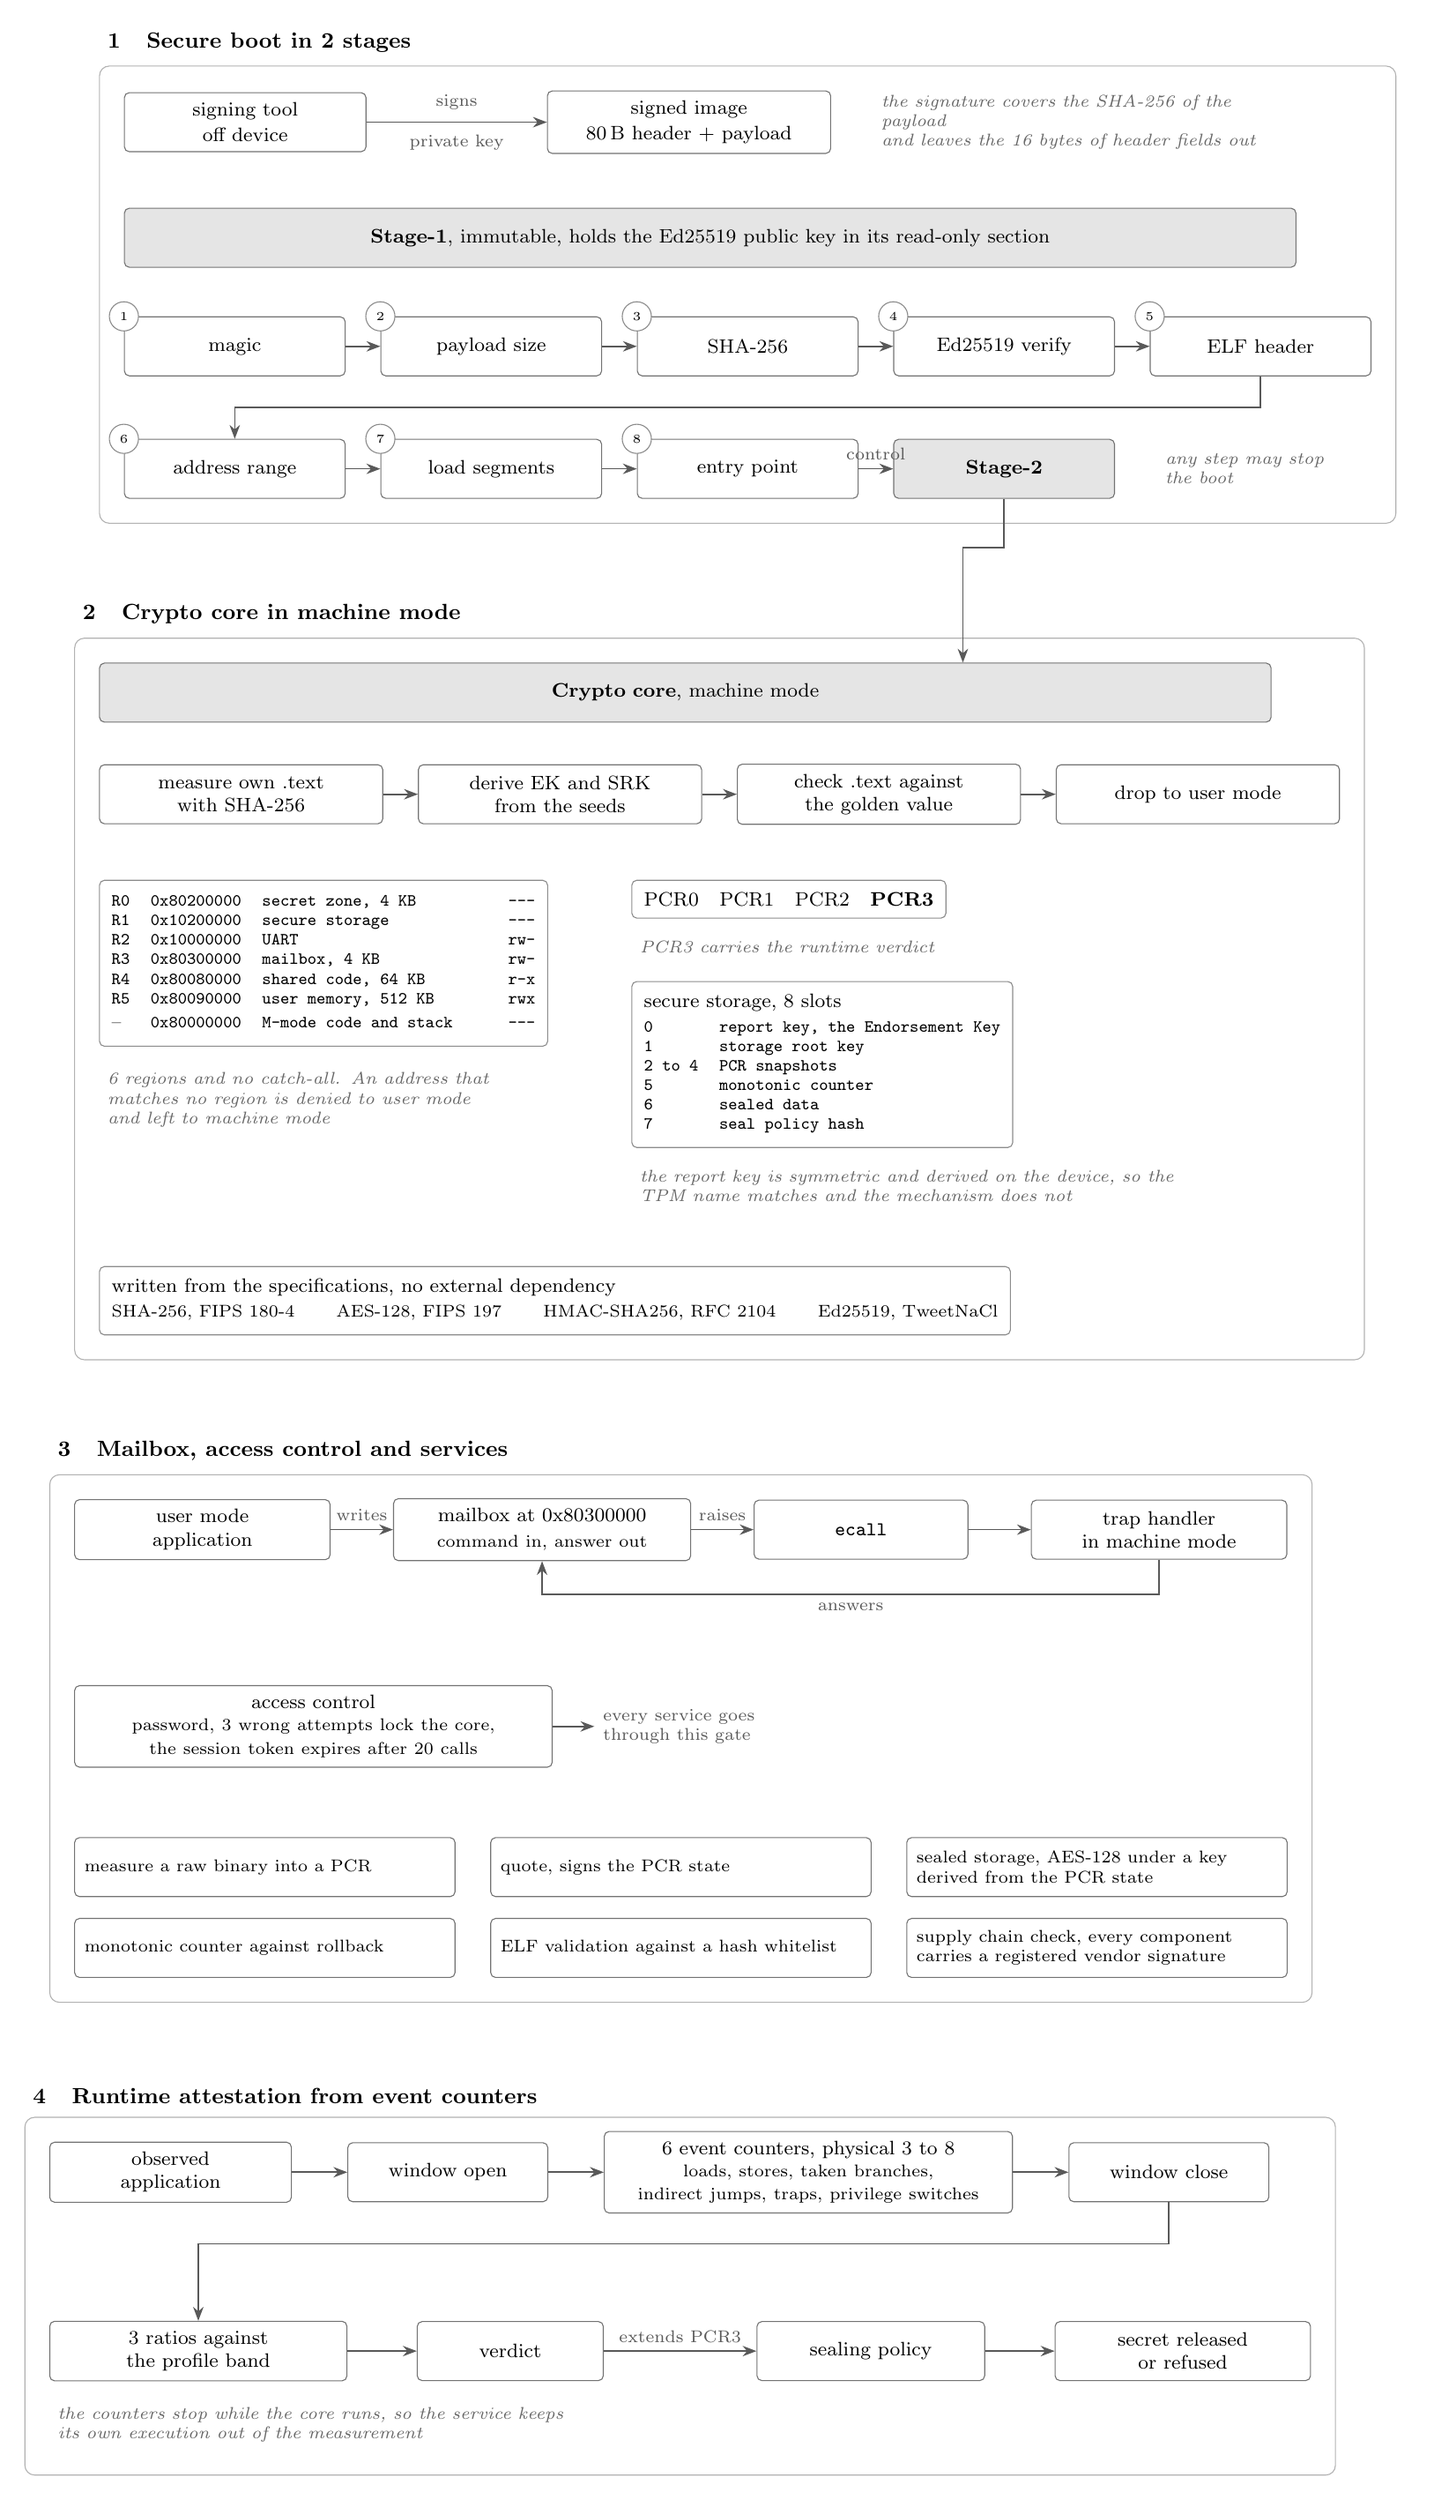
\begin{tikzpicture}[
  font=\small,
  band/.style={draw=black!30, rounded corners=4pt, inner sep=10pt},
  hdr/.style={font=\bfseries\small, anchor=south west},
  box/.style={draw=black!55, rounded corners=2pt, fill=white, align=center,
              inner sep=4pt, minimum height=8.5mm, font=\footnotesize},
  dark/.style={box, fill=black!10},
  svc/.style={box, text width=52mm, align=left, font=\scriptsize},
  panel/.style={draw=black!45, rounded corners=2pt, fill=white, inner sep=5pt},
  num/.style={draw=black!45, circle, inner sep=0pt, minimum size=4.2mm,
              font=\tiny, fill=white},
  fl/.style={-{Stealth[length=2mm]}, semithick, black!65},
  note/.style={font=\scriptsize\itshape, text=black!60, align=left}
]

%% ===================== BAND 1 : secure boot =====================
\node[box, text width=32mm] (tool) at (0,0) {signing tool\\[1pt] off device};
\node[box, text width=38mm, right=26mm of tool] (img)
  {signed image\\[1pt] 80\,B header $+$ payload};
\draw[fl] (tool) -- node[above=0.5mm, font=\scriptsize] {signs}
                   node[below=0.5mm, font=\scriptsize] {private key} (img);
\node[note, right=6mm of img.east, text width=56mm]
  {the signature covers the SHA-256 of the payload\\
   and leaves the 16 bytes of header fields out};

\node[dark, text width=166mm, below=8mm of tool.south west, anchor=north west]
  (s1) {\textbf{Stage-1}, immutable, holds the Ed25519 public key in its read-only section};

\node[box, below=7mm of s1.south west, anchor=north west, text width=29mm] (c1) {magic};
\node[box, right=5mm of c1, text width=29mm] (c2) {payload size};
\node[box, right=5mm of c2, text width=29mm] (c3) {SHA-256};
\node[box, right=5mm of c3, text width=29mm] (c4) {Ed25519 verify};
\node[box, right=5mm of c4, text width=29mm] (c5) {ELF header};

\node[box, below=9mm of c1.south west, anchor=north west, text width=29mm] (c6) {address range};
\node[box, right=5mm of c6, text width=29mm] (c7) {load segments};
\node[box, right=5mm of c7, text width=29mm] (c8) {entry point};
\node[box, right=5mm of c8, text width=29mm, fill=black!10] (s2) {\textbf{Stage-2}};

\foreach \n/\k in {c1/1,c2/2,c3/3,c4/4,c5/5,c6/6,c7/7,c8/8}
  \node[num] at (\n.north west) {\k};

\draw[fl] (c1) -- (c2); \draw[fl] (c2) -- (c3);
\draw[fl] (c3) -- (c4); \draw[fl] (c4) -- (c5);
\draw[fl] (c6) -- (c7); \draw[fl] (c7) -- (c8);
\draw[fl] (c8) -- node[above, font=\scriptsize] {control} (s2);
\draw[fl] (c5.south) -- ++(0,-4.5mm) -| (c6.north);
\node[note, right=6mm of s2.east, text width=34mm, anchor=west]
  {any step may stop\\ the boot};

\begin{scope}[on background layer]
  \node[band, fit=(tool)(img)(s1)(c1)(c5)(c6)(s2)] (b1) {};
\end{scope}
\node[hdr] at ([yshift=2pt]b1.north west) {1\quad Secure boot in 2 stages};

%% ============== BAND 2 : crypto core in machine mode ==============
\node[dark, text width=166mm, below=20mm of b1.south west, anchor=north west]
  (core) {\textbf{Crypto core}, machine mode};

\node[box, below=6mm of core.south west, anchor=north west, text width=38mm] (m1)
  {measure own .text\\ with SHA-256};
\node[box, right=5mm of m1, text width=38mm] (m2)
  {derive EK and SRK\\ from the seeds};
\node[box, right=5mm of m2, text width=38mm] (m3)
  {check .text against\\ the golden value};
\node[box, right=5mm of m3, text width=38mm] (m4)
  {drop to user mode};
\draw[fl] (m1) -- (m2); \draw[fl] (m2) -- (m3); \draw[fl] (m3) -- (m4);

\node[panel, below=8mm of m1.south west, anchor=north west] (pmp)
  {\scriptsize\ttfamily
   \begin{tabular}{@{}l@{\hspace{3mm}}l@{\hspace{3mm}}l@{\hspace{8mm}}r@{}}
   R0 & 0x80200000 & secret zone, 4 KB      & ---\\
   R1 & 0x10200000 & secure storage         & ---\\
   R2 & 0x10000000 & UART                   & rw-\\
   R3 & 0x80300000 & mailbox, 4 KB          & rw-\\
   R4 & 0x80080000 & shared code, 64 KB     & r-x\\
   R5 & 0x80090000 & user memory, 512 KB    & rwx\\[2pt]
   \textrm{--} & 0x80000000 & M-mode code and stack & ---\\
   \end{tabular}};
\node[note, below=2.5mm of pmp.south west, anchor=north west, text width=66mm]
  {6 regions and no catch-all. An address that\\
   matches no region is denied to user mode\\
   and left to machine mode};

\node[panel, right=12mm of pmp.north east, anchor=north west] (pcr)
  {\footnotesize PCR0\quad PCR1\quad PCR2\quad \textbf{PCR3}};
\node[note, below=2mm of pcr.south west, anchor=north west, text width=60mm]
  {PCR3 carries the runtime verdict};

\node[panel, below=9mm of pcr.south west, anchor=north west] (ss)
  {\scriptsize\ttfamily
   \begin{tabular}{@{}l@{\hspace{3mm}}l@{}}
   \multicolumn{2}{@{}l}{\textrm{\footnotesize secure storage, 8 slots}}\\[2pt]
   0 & report key, the Endorsement Key\\
   1 & storage root key\\
   2 to 4 & PCR snapshots\\
   5 & monotonic counter\\
   6 & sealed data\\
   7 & seal policy hash\\
   \end{tabular}};
\node[note, below=2mm of ss.south west, anchor=north west, text width=78mm] (ssnote)
  {the report key is symmetric and derived on the device, so the\\
   TPM name matches and the mechanism does not};

\node[panel, anchor=north west] (crypto)
  at ($(pmp.north west |- ssnote.south) + (0,-8mm)$)
  {\scriptsize
   \begin{tabular}{@{}l@{\hspace{6mm}}l@{\hspace{6mm}}l@{\hspace{6mm}}l@{}}
   \multicolumn{4}{@{}l}{\footnotesize written from the specifications, no external dependency}\\[2pt]
   SHA-256, FIPS 180-4 & AES-128, FIPS 197 & HMAC-SHA256, RFC 2104 &
   Ed25519, TweetNaCl\\
   \end{tabular}};

\draw[fl] (s2.south) -- ++(0,-7mm) -| ([xshift=40mm]core.north);

\begin{scope}[on background layer]
  \node[band, fit=(core)(m1)(m4)(pmp)(pcr)(ss)(crypto)] (b2) {};
\end{scope}
\node[hdr] at ([yshift=2pt]b2.north west) {2\quad Crypto core in machine mode};

%% ============== BAND 3 : mailbox and services ==============
\node[box, below=20mm of b2.south west, anchor=north west, text width=34mm]
  (app) {user mode\\ application};
\node[box, right=9mm of app, text width=40mm] (mbox)
  {mailbox at 0x80300000\\[1pt] \scriptsize command in, answer out};
\node[box, right=9mm of mbox, text width=28mm] (ecall) {\texttt{ecall}};
\node[box, right=9mm of ecall, text width=34mm] (trap)
  {trap handler\\ in machine mode};

\draw[fl] (app) -- node[above, font=\scriptsize] {writes} (mbox);
\draw[fl] (mbox) -- node[above, font=\scriptsize] {raises} (ecall);
\draw[fl] (ecall) -- (trap);
\draw[fl] (trap.south) -- ++(0,-5mm) -| node[pos=0.25, below, font=\scriptsize] {answers} (mbox.south);

\node[box, below=18mm of app.south west, anchor=north west, text width=66mm]
  (auth) {access control\\[1pt]
          \scriptsize password, 3 wrong attempts lock the core,\\
          \scriptsize the session token expires after 20 calls};
\draw[fl] (auth.east) -- ++(6mm,0) node[right, font=\scriptsize, align=left]
  {every service goes\\ through this gate};

\node[svc, below=10mm of auth.south west, anchor=north west] (v1)
  {measure a raw binary into a PCR};
\node[svc, right=5mm of v1] (v2)
  {quote, signs the PCR state};
\node[svc, right=5mm of v2] (v3)
  {sealed storage, AES-128 under a key\\ derived from the PCR state};
\node[svc, below=3mm of v1.south west, anchor=north west] (v4)
  {monotonic counter against rollback};
\node[svc, right=5mm of v4] (v5)
  {ELF validation against a hash whitelist};
\node[svc, right=5mm of v5] (v6)
  {supply chain check, every component\\ carries a registered vendor signature};

\begin{scope}[on background layer]
  \node[band, fit=(app)(trap)(auth)(v1)(v3)(v4)(v6)] (b3) {};
\end{scope}
\node[hdr] at ([yshift=2pt]b3.north west) {3\quad Mailbox, access control and services};

%% ============== BAND 4 : runtime attestation ==============
\node[box, below=20mm of b3.south west, anchor=north west, text width=32mm]
  (uapp) {observed\\ application};
\node[box, right=8mm of uapp, text width=26mm] (open) {window open};
\node[box, right=8mm of open, text width=56mm] (ctr)
  {6 event counters, physical 3 to 8\\[1pt]
   \scriptsize loads, stores, taken branches,\\
   \scriptsize indirect jumps, traps, privilege switches};
\node[box, right=8mm of ctr, text width=26mm] (close) {window close};

\node[box, below=17mm of uapp.south west, anchor=north west, text width=40mm]
  (ratios) {3 ratios against\\ the profile band};
\node[box, right=10mm of ratios, text width=24mm] (verdict) {verdict};
\node[box, right=22mm of verdict, text width=30mm] (seal) {sealing policy};
\node[box, right=10mm of seal, text width=34mm] (out)
  {secret released\\ or refused};

\draw[fl] (uapp) -- (open);
\draw[fl] (open) -- (ctr);
\draw[fl] (ctr) -- (close);
\draw[fl] (close.south) -- ++(0,-6mm) -| (ratios.north);
\draw[fl] (ratios) -- (verdict);
\draw[fl] (verdict) -- node[above, font=\scriptsize] {extends PCR3} (seal);
\draw[fl] (seal) -- (out);
\node[note, below=2.5mm of ratios.south west, anchor=north west, text width=76mm]
  (b4note) {the counters stop while the core runs, so the service keeps\\
   its own execution out of the measurement};

\begin{scope}[on background layer]
  \node[band, fit=(uapp)(close)(ratios)(out)(b4note)] (b4) {};
\end{scope}
\node[hdr] at ([yshift=2pt]b4.north west)
  {4\quad Runtime attestation from event counters};

\end{tikzpicture}
\end{document}
